\documentclass[border=4pt]{standalone}
\usepackage{tikz}
\usetikzlibrary{arrows.meta}
\definecolor{ink}{HTML}{2A2620}
\definecolor{violet}{HTML}{5A1BA6}
\definecolor{terracotta}{HTML}{A03A2C}
\definecolor{sage}{HTML}{8AA08A}
\definecolor{inkfaint}{HTML}{7A6F62}
\begin{document}
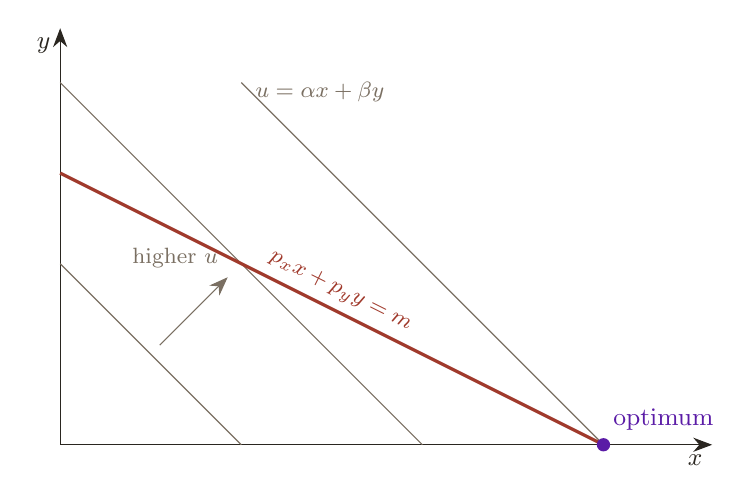
\begin{tikzpicture}[x=1.15cm,y=1.15cm,>={Stealth[length=2.4mm]},font=\small]
  % axes
  \draw[->,ink] (0,0) -- (7.2,0) node[below left]{$x$};
  \draw[->,ink] (0,0) -- (0,4.6) node[below left]{$y$};
  % indifference lines, slope -1 (steeper than budget)
  \draw[inkfaint] (2,0) -- (0,2);
  \draw[inkfaint] (4,0) -- (0,4);
  \draw[inkfaint] (6,0) -- (2,4);
  \node[inkfaint,right,font=\footnotesize] at (2.05,3.9) {$u=\alpha x+\beta y$};
  % direction of increasing utility
  \draw[->,inkfaint] (1.1,1.1) -- (1.85,1.85);
  \node[inkfaint,above left,font=\footnotesize] at (1.85,1.85) {higher $u$};
  % budget line, slope -1/2 (flatter)
  \draw[terracotta,very thick] (0,3) -- (6,0);
  \node[terracotta,rotate=-26.57,anchor=south,font=\footnotesize] at (3,1.5) {$p_x x+p_y y=m$};
  % optimum at the corner
  \fill[violet] (6,0) circle (2.4pt);
  \node[violet,above right] at (6,0.05) {optimum};
\end{tikzpicture}
\end{document}
